\documentclass{article}
\usepackage[utf8]{inputenc}
\usepackage{graphicx} 
\setlength{\parindent}{4em}
\setlength{\parskip}{1em}
\renewcommand{\baselinestretch}{1.5}

\title{BLG 354E Homework - 1}
\author{Yunus Güngör }
\date{March 2018}

\begin{document}
	
	\maketitle
	
	\section{Answers}
	
	This homework only includes answers to given questions
	
	1)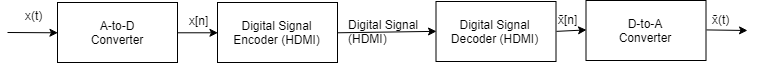
\includegraphics[scale=0.4]{q1}
	\par
	
	2)According to our class book \textit{Signal Processing First} (McCellan, Schafer, Yoder, 2003) Signals are patterns of variations that represent or encode information. Each given figure has an information with different represantation. Therefore a heartbeat record and voice record are 1 dimensional signals and an image is 2 dimensinoal signal.\par
	
	3)
	$$z^4=j$$
	$$z=-\sqrt{j}$$
	$$z=\sqrt{j}$$
	$$z=-\sqrt{j}^5$$
	$$z=\sqrt{j}^5$$
	\par
	
	4)
	$$e^{j\theta}=cos\theta+jsin\theta$$
	$$e^{j\theta}=\sum_{n=0}^{\infty}{(j\theta)^n}/n!=1+j\theta+(j\theta)^2/{2!}+(j\theta)^3/{3!}+(j\theta)^4/{4!}+...$$
	$${j\theta}^2=-\theta$$
	$${j\theta}^3=-j\theta$$
	$${js\theta}^4=+\theta$$
	$${j\theta}^5=j{\theta}^5$$
	$$e^{j\theta}=\sum{1+j\theta-(\theta)^2/{2!}-j(\theta)^3/{3!}+(\theta)^4/{4!}+...}$$
	$$e^{j\theta}=\sum{1+j\theta-(\theta)^2/{2!}+(\theta)^4/{4!}+...-j(\theta)^3/{3!}+j(\theta)^5/{5!}}+...$$
	$$e^{j\theta}=\sum{1+j\theta-(\theta)^2/{2!}+(\theta)^4/{4!}+...j(\theta-(\theta)^3/{3!}+(\theta)^5/{5!})}+...$$
	$$e^{j\theta}=cos\theta+jsin\theta$$
	\par
	
	5)
	a) A function said tob e an odd function if function shows symetry on origin.
	$$-x=f(-x)$$
	Ex:$f(x)=x^3$ , $f(x)=sin(x)$
	
	\par
	b) A function said to be an even function if function shows symetry on origin. 
	$$x=f(-x)$$
	Ex: : $f(x)=x^2$ , $f(x)=cos(x)$
	\par
	
	c)
	$$sin\theta=cos(\theta-\pi/2)$$
	$$cos(\theta+2\pi k)=cos\theta \textnormal{ , when } k \textnormal{ is integer }$$
	$$cos(-\theta)=cos\theta$$
	$$sin(-\theta)-sin(\theta)$$
	$$sin(\pi k)=0 \textnormal{ , when } k \textnormal{ is integer }$$
	$$cos(2 \pi k) = 1 \textnormal{ , when } k \textnormal{ is integer }$$
	$$cos[2 \pi (k+1/2)]=-1 \textnormal{ , when } k \textnormal{ is integer }$$
	\par
	d)i.
	$$\frac{d}{d\theta} (sin^2\theta + cos^2\theta)=\frac{d}{d\theta}1$$
	$$2sin\theta cos\theta-2cos\theta sin\theta = 0 $$
	ii.
	$$\frac{d}{d\theta}(cos(2\theta))=\frac{d}{d\theta}(cos^2\theta-sin^2\theta)$$
	$$-2sin2\theta=-2cos\theta sin\theta-2sin\theta cos\theta$$
	$$sin2\theta = 2cos\theta sin\theta$$
	iii.
	$$\frac{d}{d\theta}(sin2\theta) = \frac{d}{d\theta}(2cos\theta sin\theta)$$
	$$2cos2\theta=-2sin^2\theta +2cos^2\theta$$
	$$cos2\theta=cos^2\theta -sin^2\theta$$
	$$x=cos(\theta)+jsin(\theta)$$
	Using De Moivre's theorem:
	$$x^2=cos(2\theta) +jsin(2\theta )$$
	$$x^2=(cos(\theta) +jsin(\theta ))^2$$
	$$cos(2\theta) +jsin(2\theta)=cos^2(\theta) -sin^2(\theta )+2jcos(\theta)sin(\theta)$$
	$$cos(2\theta)=cos^2(\theta)-sin^2(\theta)$$
	$$sin(2\theta)=2sin(\theta)cos(\theta)$$
	iv.
	\begin{figure}
		\caption{Set of triangles. $EHFG$ is a rectangle. Copyrigth Lawrance Spector}
		\centering	
		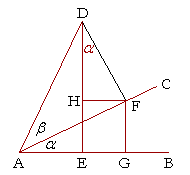
\includegraphics[scale=0.8]{q5iv}
	\end{figure}
	Using figure 1 we can derivate given formulas.
	$$sin(\alpha+\beta)=\frac{ED}{DA}$$
	Using rectangle's properties
	$$GF=EH$$
	$$HF=EG$$
	$$sin(\alpha+\beta)=\frac{FG}{AF}\frac{AF}{DA}+\frac{HD}{FD}\frac{FD}{DA}$$
	$$sin(\alpha+\beta)=sin(\alpha)cos(\beta)+cos(\alpha)sin(\beta)$$
	V.
	Using figure 1 we can derivate given formulas.
	$$cos(\alpha+\beta)=\frac{AE}{DE}$$
	Using rectangle's properties
	$$GF=EH$$
	$$HF=EG$$
	$$cos(\alpha+\beta)=\frac{AG}{AF}\frac{AF}{DA}+\frac{HF}{FD}\frac{FD}{DA}$$
	$$cos(\alpha+\beta)=cos(\alpha)cos(\beta)+sin(\alpha)sin(\beta)$$
	\par
	
	6)
	$$\sum_{k=1}^{N}A_k cos(w_o t+ \phi_k)=Re(\sum_{k=1}^{N}A_ke^{jw_0t}e^{j\phi_k})$$
	$$=Re((\sum_{k=1}^{N}A_ke^{j\phi_k})e^{jw_0t})$$
	$$=Re((Ae^j\phi)e^{jw_0t})$$
	$$=Acos(w_0t+\phi)$$
	
	\par
	
	7)
	$$z_1(t)=cos(wt-\frac{1}{3}\pi)$$
	$$z_2(t)=3cos(wt-\frac{7}{4}\pi)$$
	$$z_3(t)=2cos(wt-\frac{3}{2}\pi)$$
	$$x(t)=cos(wt-\frac{1}{3}\pi)+3cos(wt-\frac{7}{4}\pi)+2cos(wt-\frac{3}{2}\pi)$$
	\par
	a)
	$$x(t)=\sum_{k=1}^{N}A_k cos(w_o t+ \phi_k)=Re((\sum_{k=1}^{N}A_ke^{j\phi_k})e^{jw_0t})$$
	$$=Re((e^{-j\frac{1}{3}\pi} + 3e^{-j\frac{7}{4}\pi} + 2e^{-j\frac{3}{2}\pi})e^{jwt})$$
	$$=Re((0.5+0.86j+2.1-2.1j+j)e^{jwt})$$
	$$=Re((2.6-0.24j)e^{jwt})$$
	$$=Re((2.6-0.24j)e^{jwt})$$
	$$=Re(2.612e^{0.557j})e^{jwt})=2.612cos(wt+0.177\pi)$$
	\par
	b)\par
	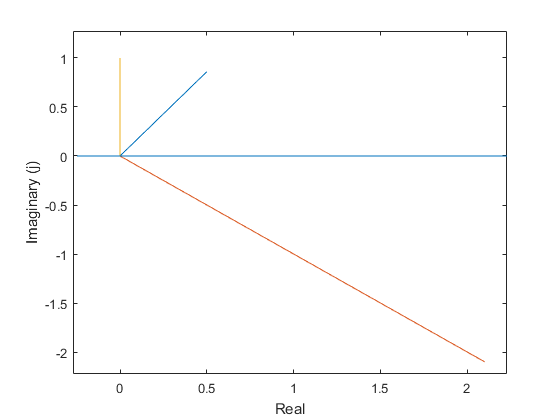
\includegraphics[scale=0.5]{q7b}
	\par
	c)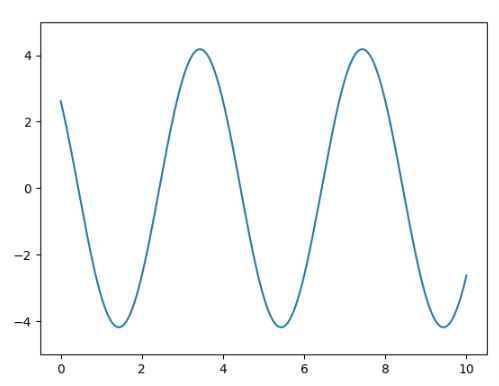
\includegraphics[scale=0.9]{q7c}
	Script to plot given graphic can be found in attachment (hw1q7c.py)
	\par
	
	8)
	$$x(t)=2+4cos(500\pi t+\frac{5}{4}\pi)-3cos(60\pi t -\frac{1}{2}\pi ) + 3cos(250\pi t - \frac{1}{4})$$
	a)\par
	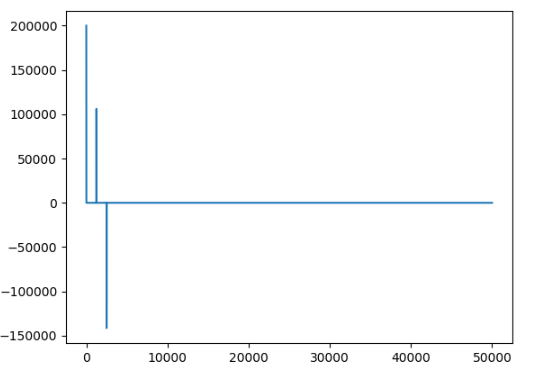
\includegraphics[scale=0.8]{q8a}
	Script to plot given graphic can be found in attachment (hw1q8a.py)
	\par
	b)
	x(t) is periodic. Period is least common mmultiple of each sinusoid's period. Those periods are respectivly, $\frac{1}{250}$ , $\frac{1}{30}$ , $\frac{1}{125}$. Therefore $x(t)$ has period of $3$. 
	$$\frac{1}{250}750=3$$
	$$\frac{1}{30}90=3$$
	$$\frac{1}{125}375=3$$
	\par
	c)It has fundamental frequency of $30$ Hertz. It has 0th and 1st harmonic 
	\par
	
	9)
	$$y_1(t)=2cos(10\pi t)$$
	$$y_2(t)=7cos(-10000 \pi t +\frac{5}{6} \pi)=7cos(10000 \pi t -\frac{5}{6} \pi$$
	\par
	a)
	$$x(t)=2cos(10\pi t)7cos(10000 \pi t -\frac{5}{6} \pi)$$
	$$=7/2(e^{j10\pi t}+e^{-j10\pi t})(e^{j 10000 \pi t -\frac{5}{6} \pi }+ e^{-j 10000 \pi t +\frac{5}{6} \pi})$$
	$$=7/2(e^{j10010\pi t -\frac{5}{6} \pi}+e^{-j 9990 \pi t + \frac{5}{6} \pi} +
	e^{j 9990 \pi t - \frac{5}{6} \pi}+e^{-j10010\pi t +\frac{5}{6} \pi}$$
	\par
	b)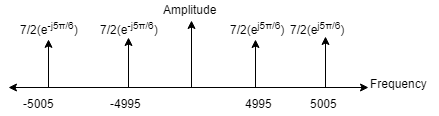
\includegraphics[scale=0.8]{q9b}
	\par
	c)
	$$x(t)=7cos(9990 \pi t - \frac{5}{6} \pi)+7cos(10010\pi t -\frac{5}{6}\pi)$$
	\par
	
	10)Two fuunctions are said to be orthogonal functions if addition of their multiplication for every value equal to zero. This means that they are orthogonal in an infinite vector space.
	
	$f(x)$ and $g(x)$ are orthogonal in $i<x<j$ if
	
	$$\int_{i}^{j}f(x)g(x)dx=0$$
	\par
	a)
	$$\int_{-L}^{L}sin(2\pi nft)sin(2\pi mft)dt=
	\frac{sin(2 \pi f t (m-n))}{4\pi(m-n)} -\frac{sin(2 \pi f t (m+n))}{4\pi(m+n)}|_{-L}^L$$
	$$=\frac{sin(2 \pi f L (m-n))}{4\pi(m-n)} -\frac{sin(2 \pi f L (m+n))}{4\pi(m+n)}+\frac{sin(2 \pi f L (m-n))}{4\pi(m-n)} -\frac{sin(2 \pi f L (m+n))}{4\pi(m+n)}=0$$
	Assuming $fL(m-n)$ and $fL(m+n)$ are integers $sin(2\pi)=0$ functions are orthogonal.
	\par
	
	b)
	$$\int_{-L}^{L}cos(2\pi nft)cos(2\pi mft)dt=
	\frac{sin(2 \pi f t (m-n))}{4\pi(m-n)} -\frac{sin(2 \pi f t (m+n))}{4\pi(m+n)}|_{-L}^L$$
	$$=\frac{sin(2 \pi f L (m-n))}{4\pi(m-n)} -\frac{sin(2 \pi f L (m+n))}{4\pi(m+n)}+\frac{sin(2 \pi f L (m-n))}{4\pi(m-n)} -\frac{sin(2 \pi f L (m+n))}{4\pi(m+n)}=0$$
	Assuming $fL(m-n)$ and $fL(m+n)$ are integers $sin(2\pi)=0$ functions are orthogonal.
	\par
	
	c)
	$$\int_{-L}^{L}sin(2\pi nft)cos(2\pi mft)dt=
	\frac{cos(2 \pi f t (m-n))}{4\pi(m-n)} -\frac{cos(2 \pi f t (m+n))}{4\pi(m+n)}|_{-L}^L$$
	$$=\frac{cos(2 \pi f L (m-n))}{4\pi(m-n)} -\frac{cos(2 \pi f L (m+n))}{4\pi(m+n)}-\frac{cos(2 \pi f L (m-n))}{4\pi(m-n)} +\frac{cos(2 \pi f L (m+n))}{4\pi(m+n)}=0$$
	Functions are orthogonal.
	
	\par
	
	11)Gibbs phenomenon is occurs when a discontinuous signal such as a square signal, represented as sum of sinusoidal functions such as Fourier series. Sum of sinusoidal functions osillates near the discontinuity and creates a bump in the shape of wave.
	
	
\end{document}
